%%%%%%%%%%%%%%%%%%%%%%%%%%%%%%%%%%%%%%%%%%%%%%%%%%%%%%%%%%%%%%%%%
% MUW Presentation
% LaTeX Template
% Version 1.0 (27/12/2016)
%
% License:
% CC BY-NC-SA 4.0 (http://creativecommons.org/licenses/by-nc-sa/3.0/)
%
% Created by:
% Nicolas Ballarini, CeMSIIS, Medical University of Vienna
% nicoballarini@gmail.com
% http://statistics.msi.meduniwien.ac.at/
%
% Customized for UAH by:
% David F. Barrero, Departamento de Automática, UAH
%%%%%%%%%%%%%%%%%%%%%%%%%%%%%%%%%%%%%%%%%%%%%%%%%%%%%%%%%%%%%%%%%

\documentclass[10pt,compress]{beamer} % Change 10pt to make fonts of a different size
\mode<presentation>

\usepackage[spanish]{babel}
\usepackage{fontspec}
\usepackage{tikz}
\usepackage{etoolbox}
\usepackage{xcolor}
\usepackage{xstring}
\usepackage{listings}

% Introduced by David
\usepackage{eurosym}

\usetheme{UAH}
\usecolortheme{UAH}
\setbeamertemplate{navigation symbols}{} 
\setbeamertemplate{caption}[numbered]

%%%%%%%%%%%%%%%%%%%%%%%%%%%%%%%%%%%%%%%%%%%%%%%%%%%%%%%%%%%%%%%%%
%% Presentation Info
\title[Videogame development team]{Videogame development team}
\author{\asignatura\\\carrera}
\institute{}
\date{Departamento de Automática}
%%%%%%%%%%%%%%%%%%%%%%%%%%%%%%%%%%%%%%%%%%%%%%%%%%%%%%%%%%%%%%%%%


%%%%%%%%%%%%%%%%%%%%%%%%%%%%%%%%%%%%%%%%%%%%%%%%%%%%%%%%%%%%%%%%%
%% Descomentar para habilitar barra de navegación superior
\setNavigation
%%%%%%%%%%%%%%%%%%%%%%%%%%%%%%%%%%%%%%%%%%%%%%%%%%%%%%%%%%%%%%%%%

%%%%%%%%%%%%%%%%%%%%%%%%%%%%%%%%%%%%%%%%%%%%%%%%%%%%%%%%%%%%%%%%%
%% Configuración de logotipos en portada
%% Opacidad de los logotipos
\newcommand{\opacidad}{1}
%% Descomentar para habilitar logotipo en pié de página de portada
\renewcommand{\logoUno}{Images/isg.png}
%% Descomentar para habilitar logotipo en pié de página de portada
%\renewcommand{\logoDos}{Images/CCLogo.png}
%% Descomentar para habilitar logotipo en pié de página de portada
%\renewcommand{\logoTres}{Images/ALogo.png}
%% Descomentar para habilitar logotipo en pié de página de portada
%\renewcommand{\logoCuatro}{Images/ELogo.png}
%%%%%%%%%%%%%%%%%%%%%%%%%%%%%%%%%%%%%%%%%%%%%%%%%%%%%%%%%%%%%%%%%

%%%%%%%%%%%%%%%%%%%%%%%%%%%%%%%%%%%%%%%%%%%%%%%%%%%%%%%%%%%%%%%%%
%% FOOTLINE
%% Comment/Uncomment the following blocks to modify the footline
%% content in the body slides. 


%% Option A: Title and institute
\footlineA
%% Option B: Author and institute
%\footlineB
%% Option C: Title, Author and institute
%\footlineC
%%%%%%%%%%%%%%%%%%%%%%%%%%%%%%%%%%%%%%%%%%%%%%%%%%%%%%%%%%%%%%%%%

\begin{document}

%%%%%%%%%%%%%%%%%%%%%%%%%%%%%%%%%%%%%%%%%%%%%%%%%%%%%%%%%%%%%%%%%
% Use this block for a blue title slide with modified footline
{\titlepageBlue
    \begin{frame}
        \titlepage
    \end{frame}
}

\institute{\asignatura}

\begin{frame}[plain]{}
   \begin{block}{Objectives}
   \begin{itemize}
        \item Understand the roles in game development
        \item First contact with the main game development problems
        \item Understand game design
		\item Introduce basic vocabulary
	\end{itemize}
	\end{block}

   \begin{block}{Bibliography}
      \begin{enumerate}
          \item  \textit{Desarrollo de Videojuegos, Arquitectura del Motor de Vieojuegos}. UCLM.
          \item Tynan Sylvester. \textit{Designing Games}. O'Reilly
          \item Wikipedia
      \end{enumerate} 
   \end{block}
\end{frame}

{
\disableNavigation{white}
\begin{frame}[shrink]{Table of Contents}
 \frametitle{Table of Contents}
 \tableofcontents
  % You might wish to add the option [pausesections]
\end{frame}
}

\section{Overview}
\begin{frame}{Overview (I)}
	\begin{itemize}
	\item Videogame development is highly multidisciplinary
	\item From a computing perspective
		\begin{itemize}
		\item Hardware, peripherals, ...
		\item Videogames software engineering, usability, gameplay, graphical computing, AI, ...
		\end{itemize}
	\item From a non-computing perspective
		\begin{itemize}
		\item Creative team: Artists, graphical designers, creatives, musicicians, level designers, ...
		\item Marketing and management
		\end{itemize}
	\item Three big teams
		\begin{itemize}
		\item Marketing: Game sales
		\item Creative and innovation: Conceptualitation of new games
		\item Production: Game implementation
		\end{itemize}
	\end{itemize}
\end{frame}

\begin{frame}{Overview (II)}
	\centering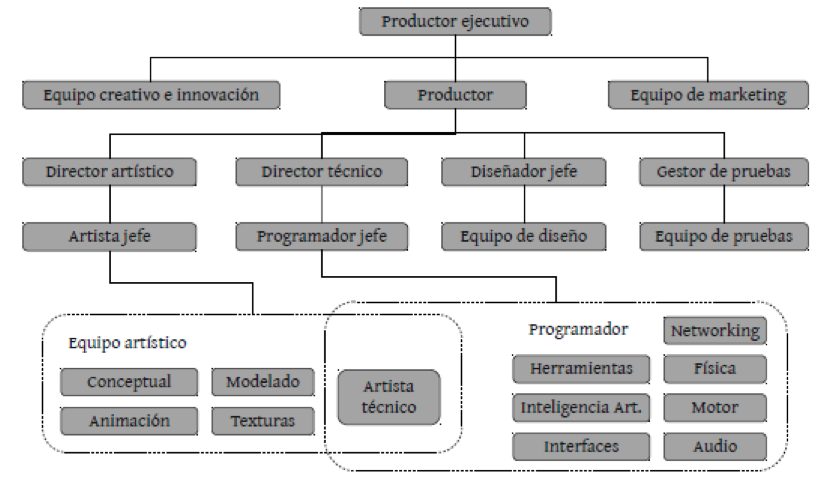
\includegraphics[width=0.9\linewidth]{figs/equipo}\\
	\tiny{Source: \textit{Desarrollo de Videojuegos, Arquitectura del Motor de Videojuegos. UCLM.}}\\
	\begin{center}
	\href{http://en.wikipedia.org/wiki/Video\_game\_development}{(More info)}
	\end{center}
\end{frame}

\section{Design team}
\begin{frame}{Design team (I)}
	\begin{itemize}
	\item They design the videogame structure
		\begin{itemize}
		\item Story, sequence of chapters, game mechanics, goals, characters, write dialogs, hint system, etc
		\end{itemize}
	\item Key concept: \alert{Level designer}
	\item It works coordinated with the engineering team
		\begin{itemize}
		\item Designers have programming tasks: NPC behavior
		\item They use high-level script languages
		\end{itemize}
	\item Script language: Interpreted language that is not compiled
		\begin{itemize}
		\item General languages: LUA, Python, Ruby
		\item Specific languages: LSL, AngelScript, GameMonkey, Io, Pawn, Squerrel, etc
		\end{itemize}
    \item Tools for level design
        \begin{itemize}
            \item Ad-hoc tools
            \item Integrated in the game engine (Unreal, Unity, etc)
            \item Specialized tools: Tiled
        \end{itemize}
	\end{itemize}
	\href{http://www.youtube.com/watch?v=KoEGyk6amq0}{(Video 1)} \href{http://www.youtube.com/watch?v=ELKi3hJkSwE}{(Video 2)}
\end{frame}

\subsection{Emotional triggers}
\begin{frame}{Design team (II)}{Emotional triggers}
    \begin{columns}
 	   \column{.1\textwidth}
 	   \column{.4\textwidth}
	Games should evoke emotions
	\begin{itemize}
		\item Learning
        \item Character arcs
        \item Challenge
        \item Social interaction
        \item Acquisition
        \item Spectacle
        \item Beauty
        \item Environment
        \item Newfangled technology
        \item Primal threats
        \item Sexual signals
	\end{itemize}
 	   \column{.45\textwidth}
		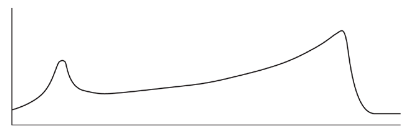
\includegraphics[width=\linewidth]{figs/emotionvariation}\\
		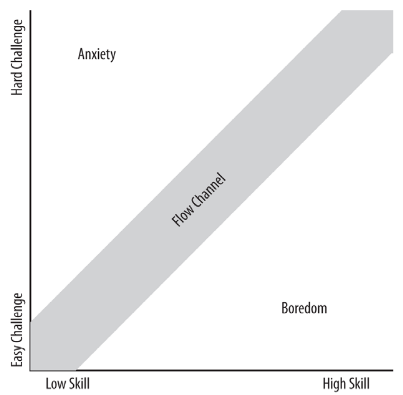
\includegraphics[width=\linewidth]{figs/flow}\\
        \tiny{Tynan Sylvester. \textit{Designing Games}. O'Reilly}
 	   \column{.1\textwidth}
    \end{columns}
\end{frame}

\subsection{Designing characters}
\begin{frame}{Design team (III)}{Designing characters}
    \begin{columns}
 	   \column{.5\textwidth}
   Main character and antagonist
   \begin{itemize}
       \item Goals
       \item Motivation
       \item Psicology
       \item History
       \item Skills
       \item Weapons
       \item Uniqueness
   \end{itemize}

 	   \column{.5\textwidth}
   Level bosses
   \begin{itemize}
        \item Characteristics
   \end{itemize}

   NPCs
   \begin{itemize}
        \item Ally
        \item Enemy
        \item Neutral
   \end{itemize}
    \end{columns}
\end{frame}

\subsection{Narrative}
\begin{frame}{Design team (IV)}{Narrative: Three acts}
   \begin{block}{Traditional three-act structure}
   \begin{itemize}
       \item Act I: Setup (\textit{introducción})
       \item Act II: Confrontation (\textit{nudo})
       \item Act III: Resolution (\textit{desenlace})
   \end{itemize}
   \end{block}
\end{frame}

\begin{frame}{Design team (V)}{Narrative: The hero's journey}
    \begin{columns}
 	   \column{.5\textwidth}
	\centering 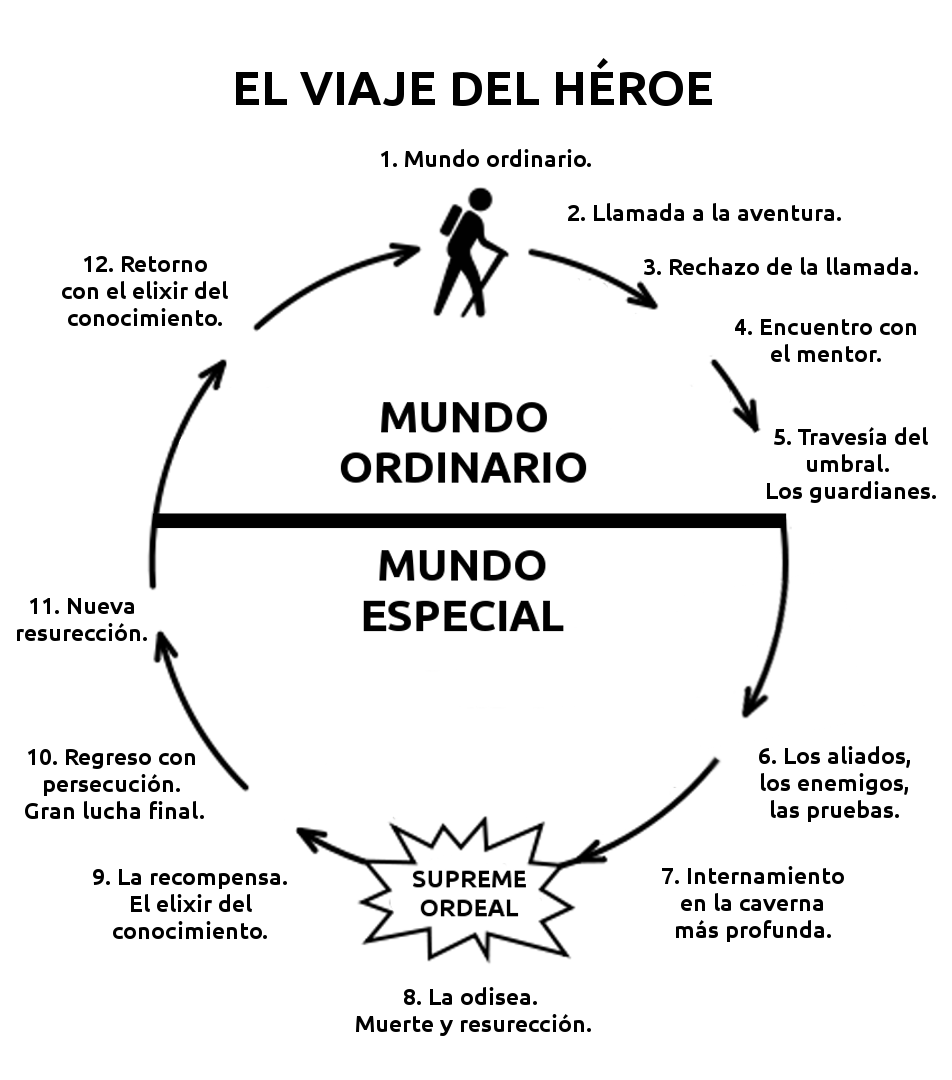
\includegraphics[width=\linewidth]{figs/heroe}
 	   \column{.5\textwidth}
	\centering 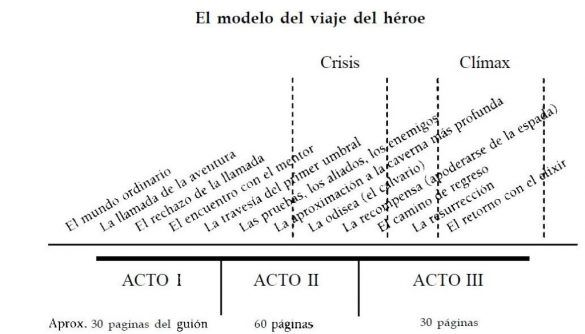
\includegraphics[width=\linewidth]{figs/actos}
    \end{columns}
	\centering \href{https://primerborrador.com/viaje-del-heroe/}{\tiny{(Source)}}\\
    \flushleft \href{https://www.youtube.com/watch?v=d1Zxt28ff-E}{(Video)}
\end{frame}

\subsection{Design document}
\begin{frame}{Design team (VI)}{Design document}
	Game design document (or \alert{GDD})
	\begin{itemize}
		\item Describes how the game is going to be
		\item Part of the creative process
		\item Used to gather funds
	\end{itemize}
	Contains
	\begin{itemize}
		\item The story
		\item Characters description
		\item Sequence of levels
		\item Game mechanics 
		\item Physics descriptions
		\item Conceptual art
	\end{itemize}
	\href{http://grumpygamer.com/maniac_mansion_design_doc}{(Maniac Mansion design document)} \href{http://playdosgamesonline.com/maniac-mansion.html}{(Maniac Mansion on-line)}
\end{frame}

\section{Artistic team}
\begin{frame}{Artistic team}
    \begin{columns}
 	   \column{.45\textwidth}
	\begin{itemize}
	\item It creates the game art
	\item Roles in the artistic team
		\begin{itemize}
		\item \href{https://www.google.es/search?espv=2&biw=1276&bih=702&tbm=isch&sa=1&q=arte+conceptual+videojuegos&oq=arte+conceptual+videojuegos&gs_l=img.3...0.0.0.116268.0.0.0.0.0.0.0.0..0.0.msedr...0...1c..64.img..0.0.0.8s-UmqTV-mo}{(Conceptual artists)}
		\item \href{https://www.google.es/search?espv=2&biw=1276&bih=702&tbm=isch&sa=1&q=modelos+3d+videojuegos&oq=modelos+3d+videojuegos&gs_l=img.3..0i24.2995.3432.0.3610.3.3.0.0.0.0.147.384.0j3.3.0.msedr...0...1c.1.64.img..2.1.122.nTWx2WYqhBc}{(Modellers)}
		\item \href{https://www.google.es/search?espv=2&biw=1276&bih=702&tbm=isch&sa=1&q=texturas&oq=texturas&gs_l=img.3..0l10.36936.37713.0.37839.8.7.0.0.0.0.208.593.0j3j1.4.0.msedr...0...1c.1.64.img..4.4.593.QFISF2dLU7U}{(Texture artists)}
		\item Illumination
		\item Animators
		\item Sound designers
		\item Actors
		\item \href{https://www.google.es/search?q=Motion+capture+actors&num=20&espv=2&source=lnms&tbm=isch&sa=X&ei=iRsZVeqlPM3fatHrgcAN&ved=0CAcQ_AUoAQ&biw=1276&bih=702}{(Motion capture actors)}
		\end{itemize}
	\end{itemize}
 	   \column{.55\textwidth}
		\centering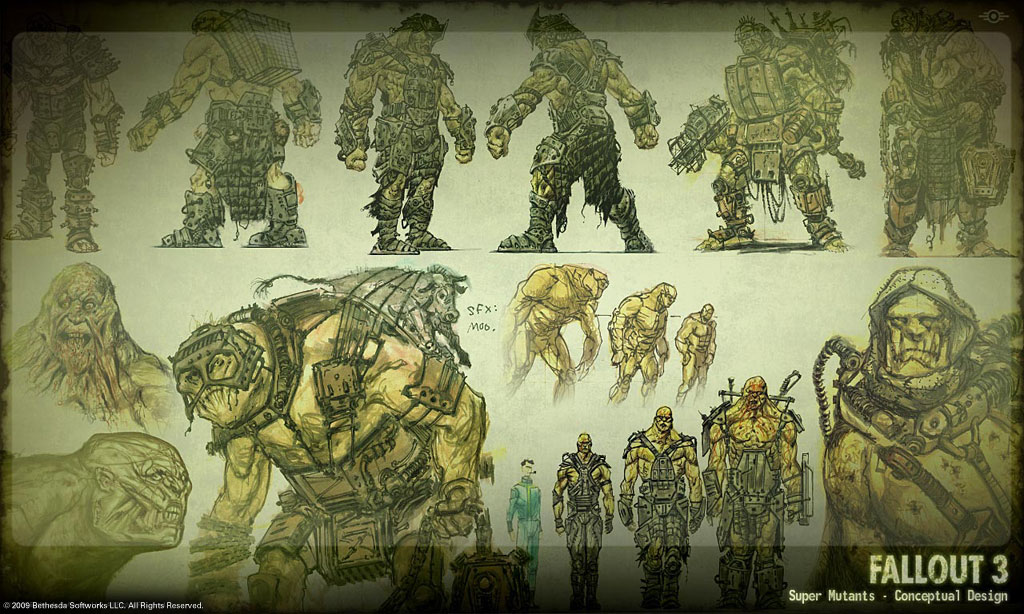
\includegraphics[width=\linewidth]{figs/concept14B}\\
		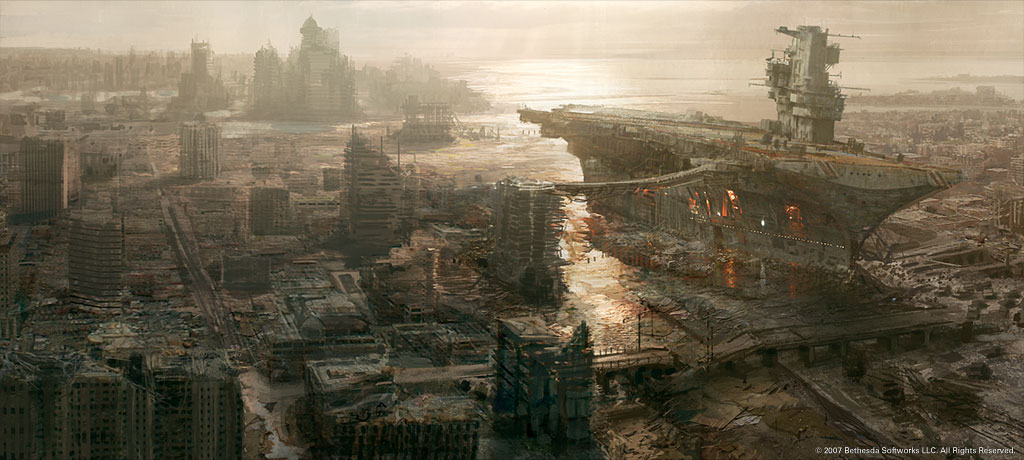
\includegraphics[width=\linewidth]{figs/fallout-3-0053}
	\end{columns}
\end{frame}

\subsection{Tools}
\begin{frame}{Artistic team}{Tools}
	\vspace{-0.2cm}
    \begin{columns}
 	   \column{.5\textwidth}
	   \begin{block}{2D design}
			Photoshop, Gimp, Illustrator, ...
		\end{block}
	   \begin{block}{3D design}
			Blender, Maya, 3D Studio Max, Lightwave, Modo, ...
		\end{block}
		\begin{block}{Video editors}
			Cinelerra
		\end{block}
	   \begin{block}{Sound editors}
			Audacity
		\end{block}
 	   \column{.5\textwidth}
	   \tiny
	   \begin{center}
		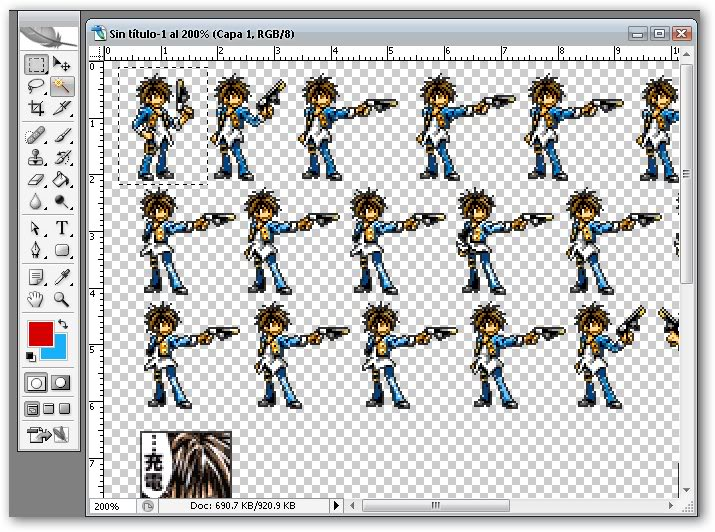
\includegraphics[width=0.8\linewidth]{figs/sshot-6}\\
		\href{http://chrisfucktheworld.blogspot.com.es/2009/06/como-hacer-animaciones-gif-con-adobe.html}{(Source)}\\
		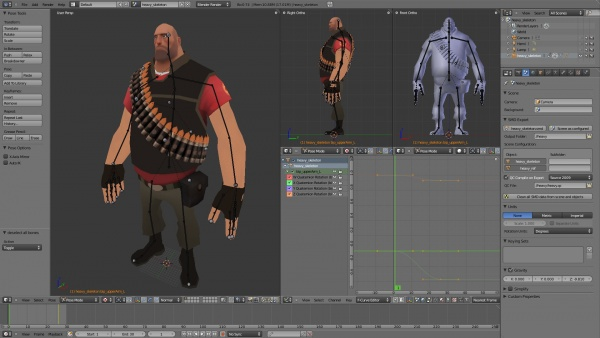
\includegraphics[width=0.8\linewidth]{figs/blender}\\
		\href{http://wiki.ikaslab.org/index.php/Dise\%C3\%B1o_3D}{(Source)}
		\end{center}
	\end{columns}
\end{frame}

\section{Engineering team}
\begin{frame}{Engineering team (I)}
	\begin{itemize}
	\item It designs and implements software
		\item Kernel programmers: Game kernel and components
			\begin{itemize}
			\item Physics, AI, graphics, sound, gameplay, scripting, UI, input processing, networking
			\end{itemize}
		\item Tools programmers: Support tools for other teams 
			\begin{itemize}
			\item Level editors
			\item Dialog editors
			\item 3D modelling
			\item NPC editors and testers
			\item Landscape generators, etc
			\end{itemize}
	\item Development tools may be published
	\end{itemize}
\end{frame}

\begin{frame}[plain]{Engineering team (II)}
    \begin{columns}
 	   \column{.5\textwidth}
		\centering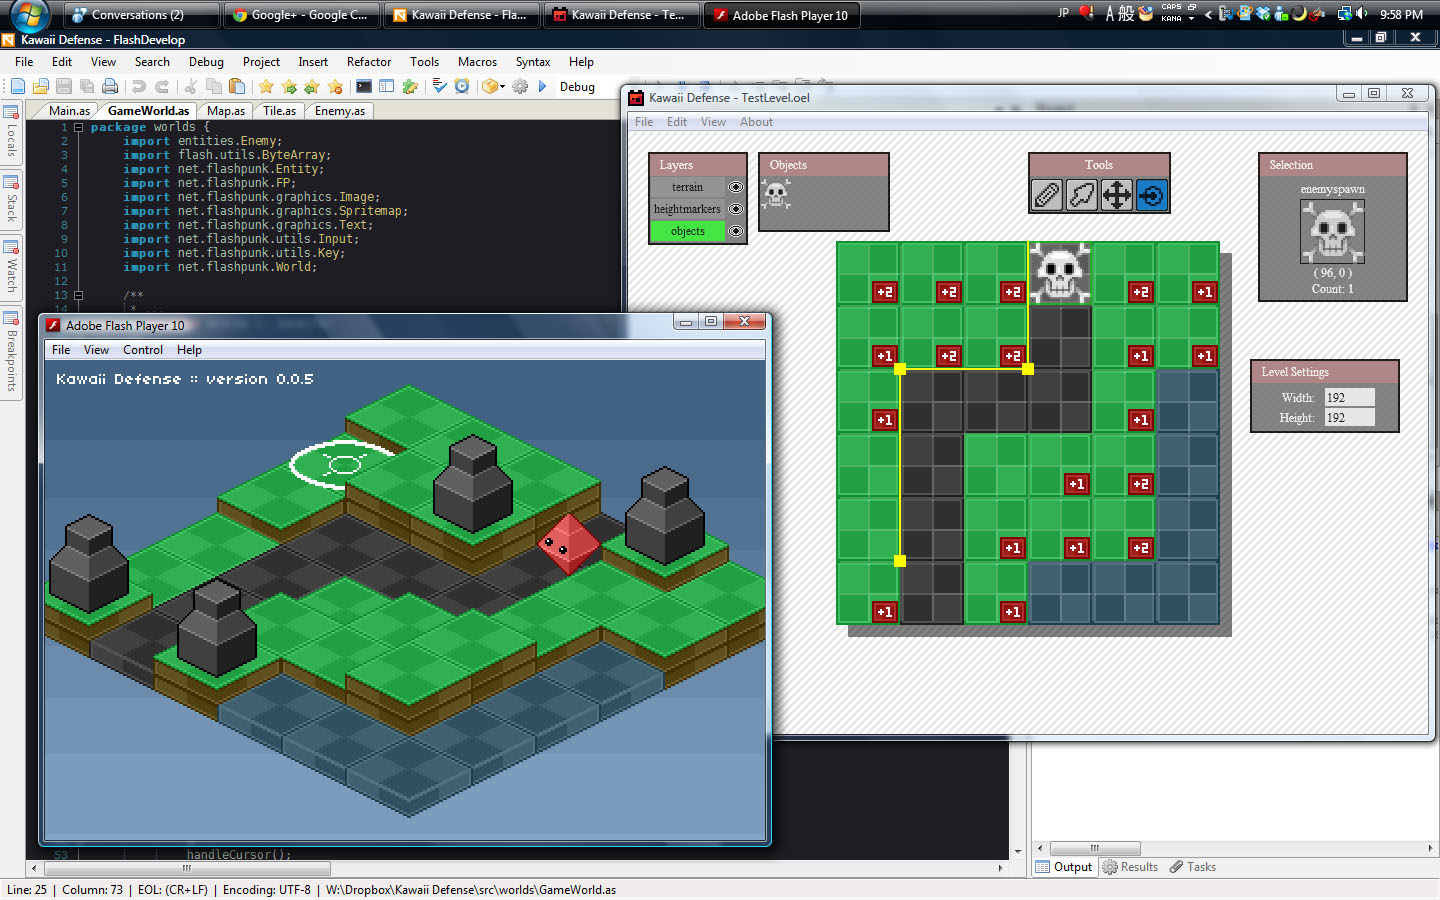
\includegraphics[width=\linewidth]{figs/devscreen2}\\
		\centering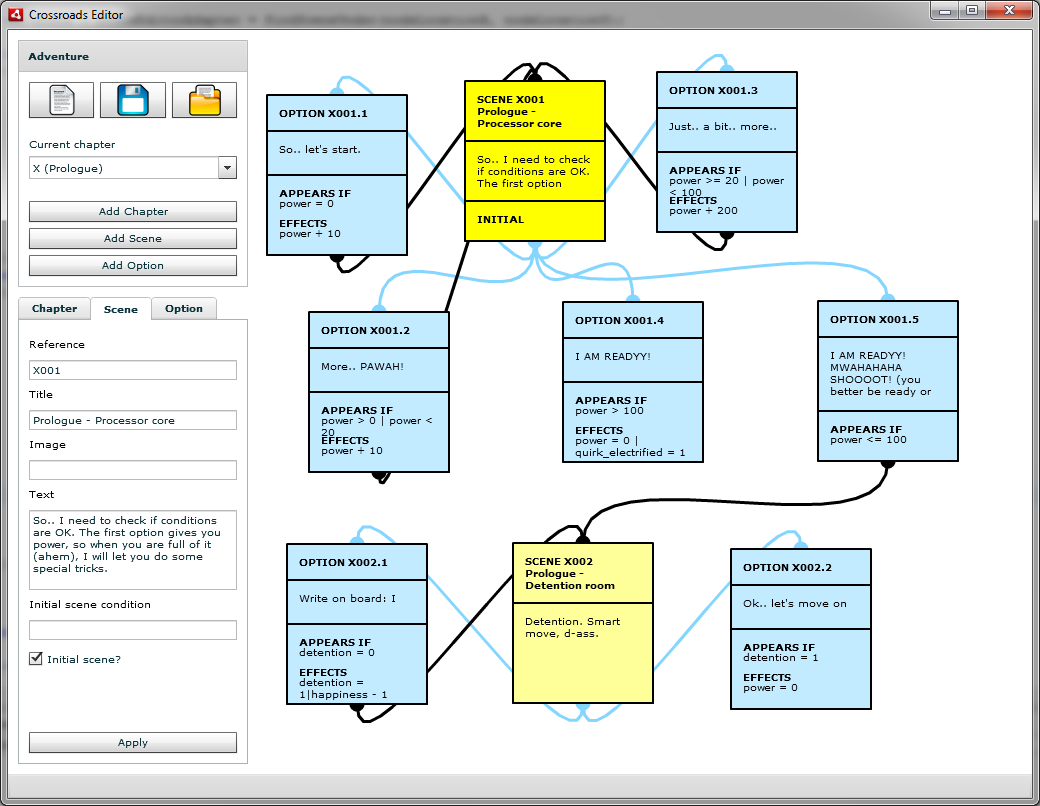
\includegraphics[width=\linewidth]{figs/crossroads_editor2}
 	   \column{.5\textwidth}
		\centering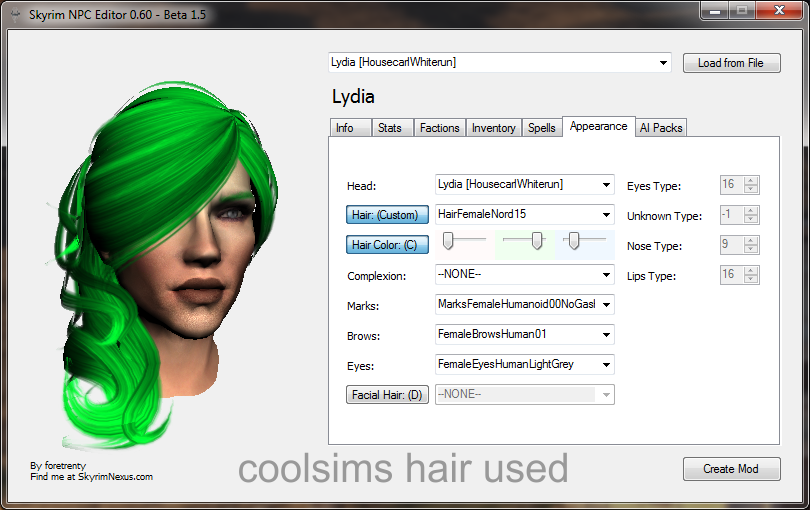
\includegraphics[width=\linewidth]{figs/npceditor}\\
		\centering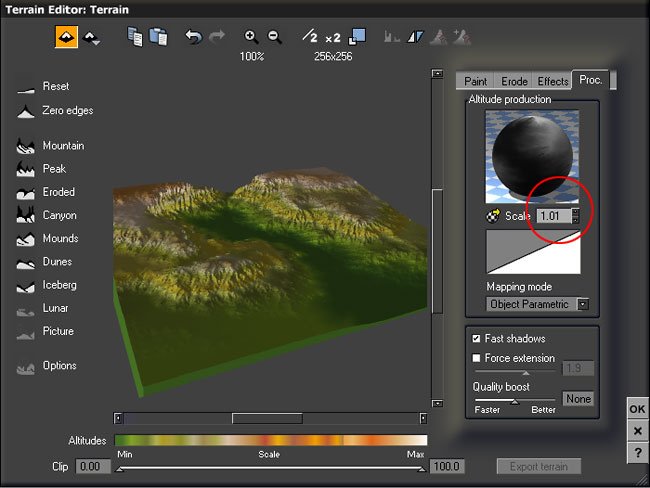
\includegraphics[width=\linewidth]{figs/geocontrol07}
		\end{columns}
\end{frame}

\subsection[Quality team]{Quality team}
\begin{frame}{Engineering team}{Quality team}
	\begin{itemize}
		\item Also known as testing, beta testing, quality control, ...
		\item Testers look for bugs
			\begin{itemize}
				\item Technical bugs
				\item Entertainment issues
			\end{itemize}
		\item Testing involves:
			\begin{itemize}
				\item Features, compatiblity, localization
				\item Active search of bugs
			\end{itemize}
		\item When a bug if found, testers must document it
			\begin{itemize}
				\item Bug tracking software: Redmine, Jira, Bugzilla, ...
			\end{itemize}
	\end{itemize}
    \href{https://www.youtube.com/watch?v=eVb_hgMeSDM}{(Fallout 4)}\\
	\href{http://en.wikipedia.org/wiki/Game\_testing}{(More info)}
\end{frame}

\end{document}
